\section{Mode 2 - Hand tracking}

\subsection{Mode description}

This mode allow the user to control directly the head of the robot. The principle is simple, the program track the finger of the user with the help of the leap motion sensor. The position is then scaled to fit in the robot moving area (over the table for instance). A command is then issued to order the robot to move to the calculated position. For testing simplicity, the mouvement are only allowed over two axes, x and y (you cannot go up), but adding a new direction to move to could be done in a matter of minutes.
One important thing one could notice is that there is no delay in the information sent to the robot. This lack a delay is due to the fact that for this particular part it doesn't matter if the robot misses a few position the mouvement being executed in a small area.
At the same time the robot is drawing, a window is opened with opencv in order to draw on the screen, the type of expected output is the following.

\begin{figure}[H]
	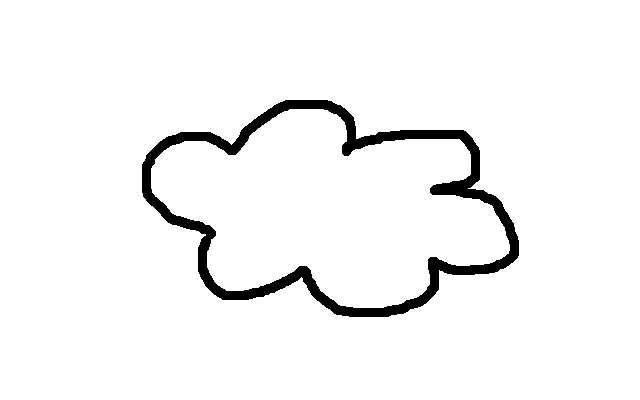
\includegraphics[scale = 0.5]{cloud}
	\centering
	\caption{Example of drawing}
	\label{fig:letter}
\end{figure}

\subsection{filter}

One of the objective of this project was to make the leap sensor less sensible to noises. There are many way to do that and many type of existing filters. But as far as our testing went a simple mean filter is more than enough to stabilize the output of the mode 2. The mean filter can be set to work on a diffrent number of position (the ... previous ones).

\begin{figure}[H]
	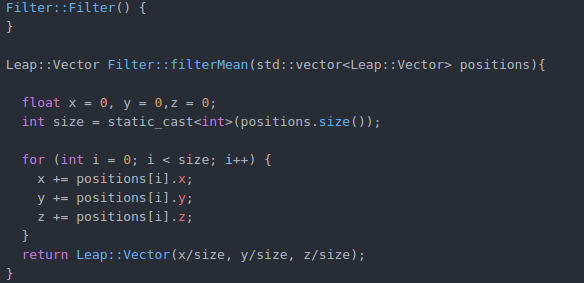
\includegraphics[scale = 0.5]{codeFilter}
	\centering
	\caption{Code of the filter}
	\label{fig:letter}
\end{figure}
